\chapter{Conclusion and future work}\label{ch:conclusion}

\begin{figure}[h!]
\centering
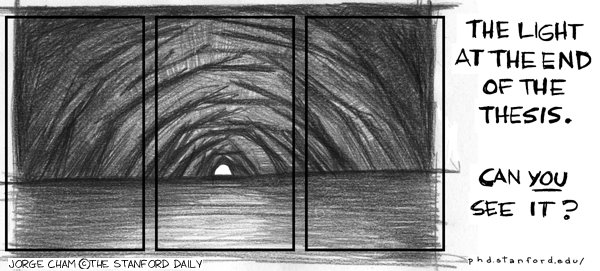
\includegraphics[width=.8\textwidth]{./gfx/Chapter07/phd051700s.jpg}
\caption{A  comic strip by Jorge Cham from his series ``Piled Higher and Deeper'' \cite{Cham}}
\end{figure}

The main goal of this thesis was to explore appearance-based methods in the novel contexts of wearable and hand-held object recognition and visual localization, with emphasis on whether biologically-inspired algorithms can have a positive impact on performance. Therefore, around this idea we defined individual hypotheses for the work described in each chapter. As means to achieve this objective we collected two large datasets; provided a thorough evaluation of baseline and custom-created image description methods; developed a biologically inspired model of place cells for visual localization and produced a prototype system for assistive localization using wearable/hand-held visual input and tactile feedback.

In this final section we will extend this summary for each of these contributions and address some future perspectives.

\section{Summary of contributions}

\begin{enumerate}
\item \textbf{Context based image retrieval (CBIR) methods for wearable and assistive applications} First, we have analysed the impact of computer vision in mobile and wearable technologies in an assistive context, providing complete studies of appearance-based methods for two key applications, hand-held object recognition of household products and indoor navigation.

\item \textbf{Artificial Place Cell Model} Second, we have provided a novel artificial place cell (APC) model for their biological counterparts found in the hippoccampus, and tested it under the same challenging conditions of indoor navigation by using a generalised regression neural network as a training mechanisms for learning a positional ground truth from a database.

\item \textbf{Prototype of an assistive application} Third, we took this previous findings to the next step and develop a prototype client-server Android application for assistive localization from wearable and hand-held devices using their visual input and a haptic feedback tablet to provide tactile cues to the location estimates. With this work we laid out the foundations for an achievable solution from the commercial perspective and stressed the importance of inclusive design.


\item \textbf{Two novel datasets} These contributions are accompanied by two important datasets, namely the SHORT dataset for hand-held object recognition and the RSM dataset of \emph{visual paths}.
\end{enumerate}

As we can see, from the computer vision application development pipeline devised in Figure ~\ref{fig:cv_dev_pipeline} we have accomplished all the stages.

\section{Concluding remarks}

\subsection{Context based image retrieval (CBIR) methods for wearable and assistive applications}

The research question for Chapters \ref{ch:chapter2},~\ref{ch:chapterSHORT},~\ref{ch:chapter4} was whether the appearance-based CBIR methods extensively used in the object recognition field could be applied to the challenging scenarios of wearable and assistive applications, with emphasis in two key applications: object recognition and visual indoor localisation. Therefore in Chapter \ref{ch:chapter2} we studied the particularities of this use case, and defined simple image matching methods and metrics and test them with prototype data so we could specify the data and performance requirements for the more thorough evaluation carried out in the following chapters.

The work described in Chapter~\ref{ch:chapter3} focuses on hand-held object recognition. We described the acquisition of the SHORT dataset and the evaluation of popular appearance-based methods aganst this dataset. The dataset proved to be extremely challenging even for algorithms that had practically solved other datasets. With the arrival of new datasets such as SHORT and ImageNet, these algorithms's performance decay, and the community had to put focus on more flexible learning methods particularly deep learning.

In Chapter~\ref{ch:chapter4} we studied another important application, indoor visual localization from hand-held and wearable cameras. We acquired another large dataset, the RSM dataset, built a benchmark and developed a series of appearance-based methods and metrics we believe are more descriptive than the current state of the art. In the benchmark, we showed how our custom methods outperform standard methods such as dense SIFT or HOG3D, but also the state of the art SLAM method for indoor scnearios, LSD-SLAM. Our best method, \textit{single frame Gabor} (SF-GABOR) achieves an average error of  We also argue that the power of SLAM resides in the robustness of its tracking mechanisms. Therefore, our methods, where no tracking was applied, can serve as a complementary tool to reduce estimation erros.


\subsection{Artificial Place Cell Model}

\subsection{Prototype of an assistive application}

\subsection{Datasets}

\subsubsection{SHORT dataset}

In the case of SHORT, we took a slightly different approach and diverged from the trend in object recognition dataset research. Instead of going towards the domain and dataset depth of big data (although our datasets are not small, containing hundreds of thousands of examples), we emphasise the need of understanding better the constraints of the problem at hand (wearable or hand-held object recognition) and also comprehend why even state-of-the art deep learning approaches that purely learn from examples find it hard to generalise outside the dataset they're being trained --and tested- on. Torralba and Efros already studied the perils of dataset bias and poor cross-dataset generalisation \cite{torralba2011unbiased} and these was one of the main motivations to build the SHORT dataset as there were no available dataset that could capture the challenges of wearable or hand-held recognition of groceries.

With the expansion of SHORT from 30 to 100 categories the category depth problem was solved, allowing for enough generalisation challenge from within the dataset. The test set, with more than, 130,000 images constitutes an extremely challenging results, with some preliminary work  being carried out in our group demonstrating the poor performance of deep learning frameworks such as Berkeley's Caffe \cite{jia2014caffe}.

\section{Future work}

Finally, we will summarise here the future work for each line of work previously described in each corresponding chapter.

\subsection{Datasets}

One might think that a straightforward future work for a dataset is just carry out an expansion. We think that this is one of the key aspects for the growth and dissemination of the data. However, we need to take into account current challenges and opportunities of crowdsourcing techniques and big data scenarios.

\subsubsection{SHORT dataset}

A large proportion of the time dedicated to the acquisition of SHORT was invested in prototypes of the acquisition set-up and trials for its testing. The intention was to have a flexible but at the same time reproducible set-up, as it can be shown in Fig. \ref{fig:acqsetup}. As the number of categories in the last version of SHORT, SHORT-100 was deemed appropriate in terms of generalisation under our testing conditions, we decided to stop its development there. However, the more categories we have in the training dataset the better for this type of benchmarks (controlled training set \textit{vs.} natural or \textit{wild} test set) to be adopted. Therefore it is important to contact large suppliers of product images to supermarket and retail chains and propose collaboration plans beneficial to both the research community (these suppliers are capable of taking our approach to scale) and for the image suppliers, as they can have an important role in acquiring the models for future improved training algorithms.

Regarding the test set, a natural expansion would consist of the setup of a web repository and the development of a retrieval mobile app so images of new grocery products could be contributed to the platform.

In this respect, there are open-source alternatives such as \cite{apple} and \cite{google} that would facilitate this task as instead of developing a dedicated app, the SHORT test set acquisition can be a project within these initiatives and attract altruist contributors that might have an interest on this sort of projects.

Alternatively, modern mobile app and web technologies allow for easy deployment of apps based on client-server communication using a RESTful architecture. By creating an API, posting images would be trivial, and the development of the client would be the final user's choice.

\subsubsection{RSM dataset}

For the RSM dataset, we envisage that a larger number of corridors could attract more users. We are currently developing synthetic data of similar-looking corridors to assess the performance of appearance-based localisation, with and without employing artificial place cell models.

Its expansion should idealy contain more variety of places, lighting conditions and overall, devices. In fact, this is an opportunity for crowdsourcing too, as a collection app or API as described in the previous section, could on its own encourage the contribution of many different devices in the process.

Finally, the acquisition of sensor data could have add huge value to the dataset. It is easy to collect sensor reading APIs are mature in mobile phone development kits, and at the same time would attract research from the sensor, ``Internet of Things'' (IoT) and big-data communities.

One of our future ideas to develop within our research group, is the modelling of similar tuning curves as the ones produced by the place cells, but on sensor data. The relationship between both sources of curves could have a huge impact in learning locations without the need of a map or even a database not obtained through crowdsourcing.

\subsection{Appearance-based methods for visual localization}

\subsection{Biologically inspired localization methods based on place cell models}
Fisher Vector as method (GMM more biologically plausible?).
\subsection{Assitive localization apps with visual input and haptic feedback}


